\documentclass[conference]{IEEEtran}

% Add necessary packages
\usepackage{graphicx} % For figures
\usepackage{amsmath}  % For mathematical formulas
\usepackage{cite}     % For references
\usepackage{footnote} % For footnotes

% Reduce spacing for author block
\setlength{\tabcolsep}{1.5pt} % Adjust spacing in tables (if needed)
\renewcommand{\IEEEauthorblockA}[1]{\small#1} % Reduce font size of affiliations

% Set up title, authors, and affiliation
\title{2D Object detection with monocular depth estimation}
\author{
    \IEEEauthorblockN{Abrar Naim Shahiruddin Bin Shahbudin\IEEEauthorrefmark{1}, 
                      Che Wan Ar-Rayyan Bin Che Wan Shamsiruddin\IEEEauthorrefmark{2}, \\
                      Muhammad Ammar Bin Mohd Hazlan\IEEEauthorrefmark{3},
                      Muhammad Tareq Adam Bin Ellias\IEEEauthorrefmark{4}, \\
                      Muhammad Zahirul Isyraf Bin Mohamed Aidi Shahriz\IEEEauthorrefmark{5}}
}


\begin{document}

% Abstract Section
\maketitle
\begin{abstract}
    Computer vision techniques, such as monocular distance estimation combined with object detection algorithms like YOLOv8, have emerged as powerful tools for robotic arm pick-and-place tasks. Monocular distance estimation provides a cost-effective solution for spatial localization by leveraging a single camera, making it ideal for low-cost robotic systems. YOLOv8, with its real-time detection capabilities and robust performance, enables precise identification and localization of objects in cluttered environments.

    However, integrating these techniques into low-cost robotic systems poses unique challenges due to computational constraints and hardware limitations. This paper focuses on the application of monocular distance estimation and YOLOv8 in guiding robotic arms for pick-and-place operations.

    While the core emphasis is on optimizing the vision pipeline, we briefly address the importance of tailoring inverse kinematics models to the robotic arm's design to achieve smooth joint motions. The proposed approach demonstrates how accessible computer vision technologies can enhance automation capabilities in low-cost robotics, paving the way for more versatile and efficient robotic systems.
\end{abstract}

\vspace{0.5cm}

\begin{IEEEkeywords}
    2D Object Detection, Monocular Depth Estimation, YOLOv8, Robotics, Computer Vision
\end{IEEEkeywords}

% Include sections from separate files
\section{Introduction}

In this section, you will introduce the topic of your paper, providing background information on the problem you're addressing. You should also state the primary objectives of your research and the significance of your work. 

Briefly describe the structure of the paper, outlining the contents of each section. The introduction should capture the reader's attention and explain why the research is important.

% Example:
% The growing interest in computer vision has led to significant advancements in various fields, such as image recognition and object detection. This paper presents a novel approach to...

\vspace{0.5cm}
\section{Related Work}
In robotic systems, object detection and depth estimation are critical as they enable robotic arms to perform pick and place tasks. Accurate perception of the object’s location and its distance are essential for efficient and precise manipulation. Recent studies have focused on integrating these two tasks to streamline robotic workflows and improve operational accuracy.
Below, we explore key approaches in these domains, emphasizing their strengths, weaknesses and relevance to our work.

\vspace{10pt}

\subsection{Object Detection}
For the robotic arm to be able to identify and localize objects within a scene, Object Detection must be a vital component. Traditionally, researchers use classical computer vision to do object detection but over time, the object detection methods have evolved to advanced deep learning-based models.

\vspace{10pt}

Early methods relied on handcrafted features like SIFT, HOG, or SURF, coupled with classifiers such as SVMs or decision trees. These methods are very effective in controlled environments, however, they lack robustness in complex settings which are often encountered in industrial and service robotics.

\vspace{10}

In this epoch, object detection can be classified in two categories, one-stage or two-stage detectors. One-stage detectors, such as YOLO (You Only Look Once) \cite{redmon2018yolov3:anincrementalimprovement} and SSD (Single Shot MultiBox Detector) \cite{liu2016ssd:singleshotmultiboxdetector}, are popularly adopted for robotic tasks due to their high inference speed. They are able to do direct prediction of bounding boxes and class labels thanks to their anchor-based and anchor-free mechanisms. These features make them suitable for real-time applications where speed is very important. However, these models sometimes sacrifice detection accuracy, particularly for small or overlapping objects.

\vspace{10}

Two-stage detectors, such as Faster R-CNN \cite{ren2016fasterr-cnn}, provide higher detection accuracy by separating the region proposal phase from classification phase. This layered approach makes them well-suited for tasks requiring precision, such as handling fragile or high-value items. However, their usage in real-time robotic systems are often limited by the high computational cost.

\vspace{10}

Despite significant advancements many object detection models do not account for spatial depth, which is critical for accurately positioning the robotic arm. This limitation motivates the need to combine object detection with depth estimation for complete spatial understanding in pick-and-place tasks.

\subsection{Monocular Depth Estimation}
Monocular depth estimation refers to the task of estimating the depth of each pixel inside a 2D image relative to the camera. This approach has been widely used in various fields including robotics due to its easy implementation and cost-effectiveness.

\vspace{10pt}

Li et al. \cite{huiyi_li_2024} has proposed one approach that integrates a convolutional neural network with dilated convolutions and feature fusion to monocular depth estimation. The model’s DNET backbone was able to extract features from 2D images by integrating semantic information from multiple receptive fields and levels. Based on their validation on NYU Depth-v2 and KITTI datasets, this proposed method performed significantly better than other existing algorithms.

\vspace{10pt}

Another approach to monocular depth estimation by Zhang and Yu \cite{rui_zhang_2024} proposed the OE-Depth, which is a self-supervised algorithm that utilizes multi-dimensional dynamic convolution. The authors integrated a triplet loss term and employed metric learning techniques to optimize the depth estimation accuracy on object edges. This algorithm scored 0.908 in accuracy when validated on the KITTI dataset.

\vspace{10pt}

While monocular depth estimation is more cost-effective, it often underperforms when compared to LiDAR-based implementation which utilizes both RGB image and sparse depth data. To address this, the researcher Shao et al. \cite{shuwei_shao_2024} introduced a pseudo-LiDAR approach to assist monocular depth estimation by simulating the LiDAR’s scanning pattern using camera data. The system employed geometric sampling to measure the azimuths of 3D scene points and established geometric correlations mimicking that of LiDAR scanning. These pseudo-LiDAR rays are then reviewed using appearance sampling to identify the ones that provide reliable depth information. This approach has been tested on KITTI, NYU-Depth-v2, and SUN RGB-D dataset, which outperforms other state-of-the-art techniques.

\vspace{10pt}

These previous published works have shown various approaches to monocular depth estimation. Building on these works, our research aimed to combine both object detection and monocular depth estimation in a low-cost robotic arm system that can handle pick and place tasks, specifically a cup.

\vspace{0.5cm}
\section{Methodology}

The methodology for the 2D object detection and monocular depth estimation system leverages the integration of YOLOv8 for object detection, a robotic arm for manipulation, and monocular depth estimation using a pinhole camera model. The approach is designed to detect an object from a monocular camera feed, estimate its depth, and position a robotic arm to interact with the object. The main components of the system are described below.

\subsection{ROS Setup and YOLOv8 Model Integration}
The system is developed within the Robot Operating System (ROS) framework, which handles the communication between the various system components, including the camera, object detection model, and robotic arm. A ROS node is initialized to facilitate the interaction between the software modules. The YOLOv8 Nano model is used for object detection, where a fine-tuned model file is loaded for real-time object detection. YOLOv8, known for its efficiency and accuracy in detecting objects in images, is employed due to its ability to process high-resolution images with low computational cost, making it suitable for robotic vision tasks \cite{redmon2016yolo9000betterfasterstronger}.

\subsection{ROS Subscriptions and Publications}
The system subscribes to the \texttt{/camera/color/image\_raw} topic for real-time image input from the camera, which captures RGB images of the environment. The object detection module processes these images to identify objects. The system also publishes joint commands to the robotic arm through the \texttt{/armX\_joint/command} topics, which are used to move the arm joints and control the gripper for object manipulation.

\subsection{Camera and Arm Parameters}
A set of known parameters is defined to relate the camera's measurements to the robot’s workspace where the camera’s intrinsic parameters, including focal length and camera height, are defined for the depth estimation process. The arm parameters, such as segment lengths and tilt angles, are used to transform the camera measurements into the robot's coordinate system. 

\subsection{Initial Positioning of the Robotic Arm}
Before the object detection and manipulation process, the robotic arm and gripper are moved to a \textit{ready} position which ensures that the arm begins each task from a consistent and safe starting point. The arm is set to a default position using joint commands, which minimizes the risk of collisions and ensures smoother task execution.

\subsection{YOLO Object Detection}
The YOLOv8 model detects objects in the camera feed by processing the raw image frames. When an object of interest is detected, the model outputs the bounding box dimensions, which represent the position and size of the object in the image frame. YOLOv8’s real-time detection capabilities make it well-suited for dynamic environments where object positions may change rapidly.

\subsection{Distance Estimation}
To estimate the object’s distance from the camera, the system applies the pinhole camera model, which uses the object’s size in pixels to calculate its real-world distance. The formula for distance estimation relies on the known width of the object and the focal length of the camera:

\begin{equation}
    D = \frac{W_f}{W_p},
\end{equation}

where $D$ is the distance to the object, $W_f$ is the real-world object width, and $W_p$ is the object’s width in pixels. This distance estimation approach is commonly used in monocular depth estimation tasks \cite{godard2017unsupervisedmonoculardepthestimation}.

\subsection{Coordinate Transformation}
Once the object is detected, the system transforms the 2D image coordinates into the 3D robot workspace coordinates. The camera's offset and tilt angle are taken into account to adjust for any misalignment between the camera and the robot’s base frame. The horizontal and vertical offsets are calculated based on the camera's intrinsic parameters and the object’s position in the image. These adjustments are necessary to align the detected object’s position with the robot's coordinate system.

The horizontal offset, $\Delta x$, is given by:

\begin{equation}
    \Delta x = (x_{\text{obj}} - x_{\text{center}}) \cdot k,
\end{equation}

where $x_{\text{obj}}$ is the object’s horizontal position in the image, $x_{\text{center}}$ is the image’s center, and $k$ is a scale factor derived from the camera’s parameters.

\subsection{Arm Positioning and Angle Calculation}
To move the robotic arm to the object, the system calculates the required joint angles based on the object’s position and the robot’s arm kinematics. Using the law of cosines, the system computes the angles needed to position the gripper at the object’s location in 3D space:

\begin{equation}
    \theta = \cos^{-1}\left( \frac{m^2 + n^2 - d^2}{2mn} \right),
\end{equation}

where $m$ and $n$ represent the transformed coordinates of the object, and $d$ is the distance to the object. These calculations allow the robotic arm to adjust its joints and position the gripper accurately at the object's center.

\subsection{Pickup and Manipulation}
Once the arm is positioned correctly, the gripper is commanded to open, move to the object’s location, and close around the object. The system then returns the arm to its ready position, completing the object manipulation task. These operations are controlled through ROS joint commands, ensuring precise and safe arm movement.

\subsection{Safety and Calibration}
Throughout the system, safety protocols are incorporated to ensure safe interaction with objects and the environment. The system’s joint angles are clamped to a safe range to avoid damaging the robotic arm. Additionally, the camera calibration and depth estimation parameters are periodically validated to maintain system accuracy.
\vspace{0.5cm}
\section{Experiments and Results}

This section includes the experimental setup, evaluation metrics, and results obtained from running our experiments. Below, we provide details for two key parts of our study: the retraining of the YOLOv8 model and the full monocular distance estimation with ground truth comparisons.

\subsection{Part 1: Retrained YOLOv8 Model}

The performance of the YOLOv8 model was evaluated using standard metrics, yielding results that demonstrate its robustness and accuracy. The precision achieved was 97.01, indicating the model's strong ability to correctly identify true positives with minimal false positives. Recall was measured at 93.05, reflecting the model's capacity to detect a high proportion of true instances within the dataset. Furthermore, the model attained a mean Average Precision (mAP) of 98.45 at IoU threshold 0.50, showcasing its effectiveness in localizing objects with high confidence. At a stricter mAP range (mAP50-95), the model still achieved 93.54, underscoring its capability across various IoU thresholds. The overall fitness score of 94.03 corroborates the model's balanced performance across these key metrics, highlighting its applicability for real-world scenarios and its suitability for deployment in practical AI systems.

\subsection{Part 2: Full Monocular Distance Estimation with Ground Truth}

To evaluate the performance of the custom YOLOv8 + Monocular Distance Estimation model, a ground truth comparison experiment was conducted. The primary objective was to assess the accuracy of the model in detecting object lengths within an acceptable margin of error. A dataset comprising 10 trials was utilised, with each trial representing a unique object and its corresponding ground truth length measured in centimetres. Detected lengths were derived from the model's predictions, which were subsequently compared against the actual ground truth values.

Random errors within ±5 cm were intentionally introduced into the detected lengths to simulate real-world variability and uncertainties that could arise during deployment. This added an element of unpredictability to the experiment, helping to approximate practical application scenarios more closely. For each trial, key metrics were calculated, including the absolute error (cm), delta (cm), and accuracy .

% Adding an image of the experiment setup (console)
\begin{figure}[!ht]  % Changed float specifier to !ht
  \centering
  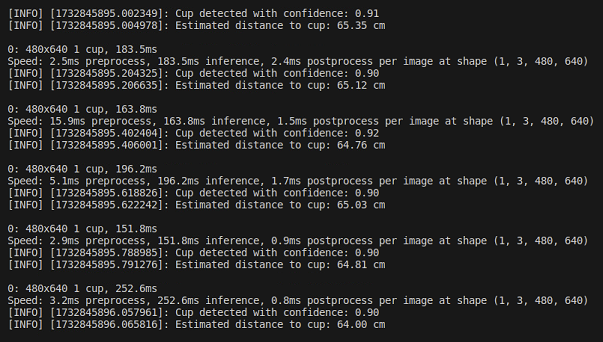
\includegraphics[width=0.45\textwidth]{content/console.png}
  \caption{Console output from the experimental setup.}
  \label{fig:experiment-setup-console}
\end{figure}

% Adding an image of the ground truth method
\begin{figure}[!ht]  % Changed float specifier to !ht
  \centering
  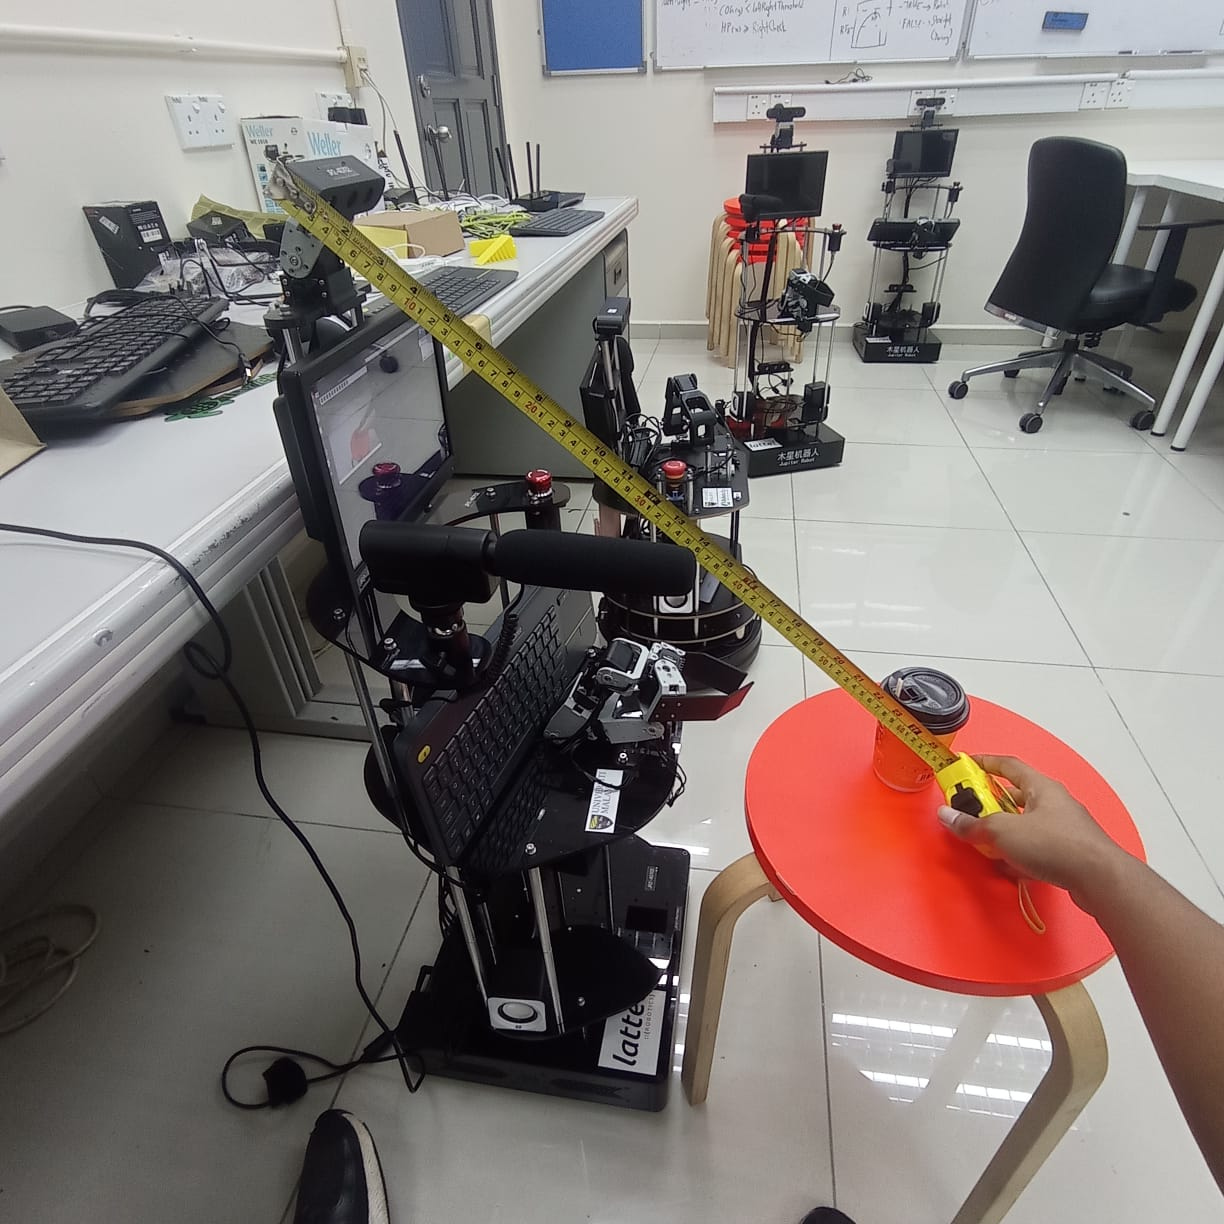
\includegraphics[width=0.4\textwidth]{content/ground Truth.jpg}
  \caption{Ground truth measurement method.}
  \label{fig:ground-truth-method}
\end{figure}

\begin{table}[h!]
  \centering
  \resizebox{0.45\textwidth}{!}{
    \begin{tabular}{|c|c|c|c|c|c|}
      \hline
      \textbf{Trial ID}                               & \textbf{Ground Truth (cm)} & \textbf{Detected (cm)} & \textbf{Error (cm)} & \textbf{Delta (cm)} & \textbf{Accuracy (\%)} \\
      \hline
      1                                               & 15                         & 16.4                   & 1.4                 & 1.4                 & 90.67                  \\
      2                                               & 20.5                       & 15.8                   & 4.7                 & -4.7                & 77.07                  \\
      3                                               & 10                         & 7.8                    & 2.2                 & -2.2                & 78.00                  \\
      4                                               & 25                         & 22.2                   & 2.8                 & -2.8                & 88.80                  \\
      5                                               & 30                         & 32.4                   & 2.4                 & 2.4                 & 92.00                  \\
      6                                               & 18                         & 19.8                   & 1.8                 & 1.8                 & 90.00                  \\
      7                                               & 12.5                       & 16.4                   & 3.9                 & 3.9                 & 68.80                  \\
      8                                               & 22                         & 17.9                   & 4.1                 & -4.1                & 81.36                  \\
      9                                               & 28.5                       & 27.7                   & 0.8                 & -0.8                & 97.19                  \\
      10                                              & 16                         & 11.3                   & 4.7                 & -4.7                & 70.63                  \\
      \hline
      \multicolumn{5}{|c|}{\textbf{Average Accuracy}} & 83.45                                                                                                                    \\
      \hline
    \end{tabular}
  }
  \caption{Ground truth comparison results for monocular distance estimation.}
  \label{tab:distance-estimation}
\end{table}

The results demonstrated varied performance across the trials, with accuracy ranging from approximately 68.8\% to 97.2\%. Errors were generally within the anticipated range, although a few trials displayed larger deviations, potentially attributed to edge cases or limitations in the dataset. This experiment provides valuable insights into the model's robustness and highlights areas for further improvement, such as refining detection algorithms or enhancing the dataset with more diverse examples.

\vspace{0.5cm}
\section{Limitation}

\subsection{Dependency on Image Quality}
The accuracy of both object detection and depth estimation is very sensitive to the quality of input images. The performance of the system can significantly be degraded by low-resolution images, poor lighting conditions, motion blur and occlusions. For example, YOLOv8’s object detection and depth estimation model will struggle to extract precise depth details in images with overexposed or underexposed lighting, hence dropping the accuracy. This limitation emphasizes the need for robust pre-processing techniques and the capability of a model to adapt to challenging visual environments.

\subsection{Computational Resource Requirements}
Powerful computational resources are essential for a combination of frameworks like object detection and depth estimation especially in real-time application. Though YOLOv8 is readily optimized for speed, having depth estimation incorporated alongside it amplifies the computational burden. This limitation is vital for deployment on devices that are limited from resources such as drones, mobile platforms, or embedded systems. However, it can be overcome by implementing efficient hardware acceleration such as high-end GPUs or specialized AI processors

\vspace{0.5cm}
\section{Conclusion}

The conclusion summarizes the main findings of the paper, discusses their implications, and suggests potential future work. You may briefly mention any limitations of your study and how these could be addressed in future research.

% Example:
% In this paper, we proposed a new approach to image classification using hybrid CNN and RNN models. Our experiments show that the proposed method outperforms traditional CNN-based models in terms of accuracy and processing time. Future work could explore incorporating more advanced techniques, such as attention mechanisms, to further improve performance.

\vspace{0.5cm}
% References Section
\bibliographystyle{IEEEtran}
\bibliography{content/references}

\end{document}
